\documentclass[12pt,a4paper]{article}
\usepackage{microtype}
\usepackage{amsfonts}
\usepackage{amsthm}
\usepackage{graphicx}

\newcommand{\dpar}[1]{\left(#1\right)}

\newcommand{\N}{\mathbb{N}}
\newcommand{\R}{\mathbb{R}}

\theoremstyle{definition}
\newtheorem{ex}{Exercise}[section]

\title{Physics 1: Class 5}
\author{Max Jauregui}

\begin{document}
\maketitle

\section{Constant acceleration (continuation)}

Figure~\ref{fig:mruv} shows the $v$ vs $t$ and $x$ vs $t$ graphs for a motion of a particle with constant acceleration.

\begin{figure}[ht]
  \centering
  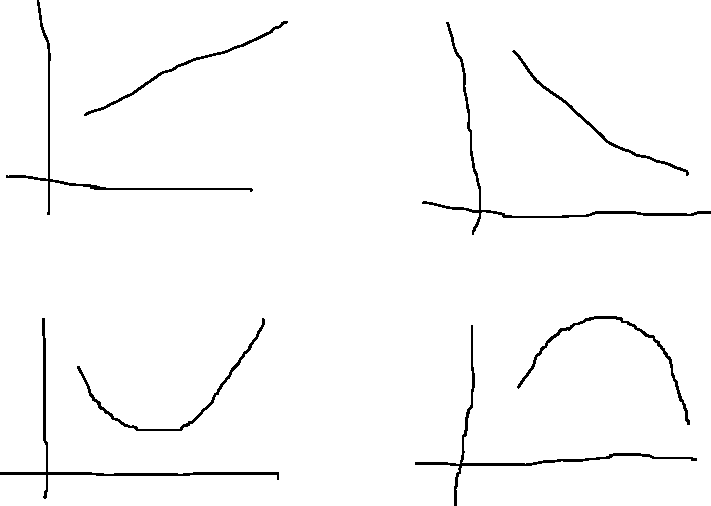
\includegraphics[width=0.5\textwidth,keepaspectratio]{figures/mruv.pdf}
  \caption{$v$ vs $t$ and $x$ vs $t$ graphs for the motion of a particle eith constant acceleration.}
  \label{fig:mruv}
\end{figure}

\begin{ex}
  A car moves with a constant velocity of $90\,\mathrm{km/h}$. In a
  certain instant the driver of the car puts the brakes on and the car
  travels $60\,\mathrm{m}$ until it stops. Assuming constant
  acceleration, find the acceleration of the car? \emph{Answer:}
  $-5{,}21\,\mathrm{m/s^2}$.
\end{ex}

\begin{ex}
  A plane initially at rest has a uniform acceleration and travels
  $800\,\mathrm{m}$ in order to take off, which it does with a
  velocity of $360\,\mathrm{km/h}$. How much time does the plane take
  to take off? \emph{Answer:} $16\,\mathrm{s}$.
\end{ex}

\begin{ex}
  A car moves with a constant velocity of $36\,\mathrm{km/h}$. When
  the car is at a distance of $60\,\mathrm{m}$ from traffic lights,
  the traffic lights turn yellow and the driver presses on the
  accelerator in order to run it. Taking into account that the
  reaction time of the driver is $0{,}6\,\mathrm{s}$, calculate the
  minimum value of the acceleration of the car in order to run the
  yellow traffic light, knowing that it lasts $4\,\mathrm{s}$. \emph{Answer:} $1{,}75\,\mathrm{m/s^2}$.
\end{ex}

\section{Free fall}

In this case $|a|=g=9{,}8\,\mathrm{m/s}$. Usually we use the $y$ axis
instead of$x$ axis. If the $y$ axis point upwards, $a=-g$; otherwise
$a=g$.

\begin{ex}
  A particle is initially at rest at height $h$ from the ground. How
  much time it will take to reach the ground? What will be its
  velocity in this moment?
\end{ex}

\end{document}
